This method enables the estimation of a vehicle’s 3D position and orientation from a single image, under the assumption of known intrinsic camera parameters and a simplified vehicle model. The approach relies on the identification of symmetric and well-localized features—typically the rear lights and the corners of the license plate—which are assumed to lie on the vehicle's rear plane. By exploiting known real-world distances between these features, it is possible to triangulate their positions in 3D space and reconstruct a rear-facing coordinate frame aligned with the vehicle geometry. The final output is a 3D bounding box that approximates the vehicle's occupied space. While this method requires only a single frame, its performance is highly sensitive to feature localization accuracy and the presence of sufficient perspective distortion in the image.

\subsection{Theoretical Foundations}
The mathematical framework underlying the method is founded on three pillars of projective geometry and photogrammetry.

\subsubsection{Pinhole Camera Model and Back-Projection}
A standard pinhole camera model is adopted, where the transformation from a 3D point in the camera space, $\mathbf{P} = [X, Y, Z]^T$, to an image point in homogeneous coordinates, $\tilde{\mathbf{x}} = [u, v, w]^T$, is described by the intrinsic matrix $K \in \mathbb{R}^{3 \times 3}$:
\[
\lambda \tilde{\mathbf{x}} = K \mathbf{P}
\]
where $\lambda$ represents the scene depth. The inverse operation, or \textbf{back-projection}, is essential for 3D reconstruction. Given an image point $\mathbf{x}_{pix}$, its homogeneous coordinates $\tilde{\mathbf{x}}$ are mapped to a 3D directional ray $\mathbf{d}$ in the camera space, according to the relation:
\[
\mathbf{d} = K^{-1} \tilde{\mathbf{x}}
\]
This vector $\mathbf{d}$ defines the line on which the 3D point $\mathbf{P}$ lies, but not its exact position along it.

\subsubsection{Triangulation with Geometric Constraints}
To resolve the depth ambiguity, a metric constraint is introduced, namely a known real-world distance such as the license plate width, $w_{plate}$. Given two image points $p_0$ and $p_1$ and their corresponding normalized 3D rays $\mathbf{d}_0$ and $\mathbf{d}_1$, they form a triangle with the camera center. The angle $\theta$ between the two rays can be calculated via the dot product:
\[
\theta = \arccos(\mathbf{d}_0 \cdot \mathbf{d}_1)
\]
Assuming that the two 3D points $\mathbf{P}_0$ and $\mathbf{P}_1$ are at approximately the same depth from the camera, the triangle formed by $\mathbf{P}_0$, $\mathbf{P}_1$, and the camera center can be approximated as isosceles. The average depth $d$ can then be estimated geometrically:
\[
d_{approx} = \frac{w_{plate}}{2 \sin(\theta / 2)}
\]
This estimate is subsequently refined to ensure that the Euclidean distance between the reconstructed 3D points, $\mathbf{P}_0 = d_0 \mathbf{d}_0$ and $\mathbf{P}_1 = d_1 \mathbf{d}_1$, exactly satisfies the constraint $\|\mathbf{P}_1 - \mathbf{P}_0\| = w_{plate}$.

\subsubsection{Vanishing Point Geometry}
The vehicle's orientation is recovered by exploiting the properties of vanishing points. In projective geometry, parallel lines in 3D space appear to converge to a single point on the image plane, known as the vanishing point. By identifying two or more lines on the image known to be parallel in reality (e.g., the top and bottom edges of the license plate), their intersection point $\mathbf{v_p}$ can be computed. The back-projection of $\mathbf{v_p}$ yields a 3D vector $\mathbf{v}_{dir}$ that indicates the direction of these parallel lines in the camera space, corresponding to the vehicle's longitudinal axis.
\[
\mathbf{v_p} = l_1 \times l_2 \quad \implies \quad \mathbf{v}_{dir} = K^{-1} \mathbf{v_p}
\]

\subsubsection{Algorithmic Pipeline}
The implementation of the method follows a defined sequence of operations.

\begin{enumerate}
    \item \textbf{Preprocessing and Feature Extraction}: The image is corrected for optical distortions using known calibration parameters ($K$, \texttt{dist}). Subsequently, four coplanar keypoints are extracted: two corners of the license plate (\texttt{TL}, \texttt{TR}) and the two taillights (\texttt{L2}, \texttt{R2}). The coordinates of these points are also undistorted.

    \item \textbf{3D Point Reconstruction}: The \texttt{triangulate\_plate\_points} function implements the constrained triangulation described above to compute the 3D coordinates, $\mathbf{P}_0$ and $\mathbf{P}_1$, of the license plate corners.

    \item \textbf{Vanishing Point Estimation}: The function \texttt{compute\_vanishing\_direction} calculates the intersection of two lines in the image: the first connects the license plate corners (points \texttt{TL} and \texttt{TR}), and the second connects the taillights (points \texttt{L2} and \texttt{R2}). These lines, assumed to be parallel in the real world, intersect in the image due to perspective projection. Their intersection defines a vanishing point $\mathbf{v_p}$ in the image plane, which is then back-projected into a 3D direction vector $\mathbf{v}_{dir} = K^{-1} \mathbf{v_p}$ that approximates the vehicle's forward direction in the camera coordinate frame.

    \item \textbf{Vehicle Coordinate Frame Construction}: The \texttt{build\_vehicle\_frame} function establishes a local coordinate system attached to the vehicle.
    
    \begin{itemize}
        \item \textbf{X-axis}: Defined as the unit vector connecting the two 3D license plate points, $\mathbf{x}_{axis} = \text{normalize}(\mathbf{P}_1 - \mathbf{P}_0)$.
        \item \textbf{Y-axis}: Calculated from the vanishing point direction $\mathbf{v}_{dir}$, made orthogonal to $\mathbf{x}_{axis}$ through a Gram-Schmidt orthogonalization process.
        \item \textbf{Z-axis}: Obtained via the cross product $\mathbf{z}_{axis} = \text{cross}(\mathbf{x}_{axis}, \mathbf{y}_{axis})$ to form a right-handed coordinate system.
        \item \textbf{Origin}: Placed at the center of the license plate segment, then translated along the local Z-axis.
        \item \textbf{Rotation Matrix}: The vehicle's rotation matrix $R$ relative to the camera is constructed by stacking the three axes as columns: $R = [\mathbf{x}_{axis} | \mathbf{y}_{axis} | \mathbf{z}_{axis}]$.
    \end{itemize}

    \item \textbf{3D Bounding Box Generation}: The 8 vertices of the cuboid are defined in the vehicle's local coordinates, based on its known dimensions. Each local vertex $\mathbf{p}_{local}$ is then transformed into the camera's coordinate system using the estimated pose (rotation $R$ and translation origin): $\mathbf{p}_{camera} = R \mathbf{p}_{local} + \text{origin}$.
\end{enumerate}

\subsection{Results and Discussion}
The outcome of this method is shown in Figure~\ref{fig:method1_result}. While the reconstructed bounding box follows the expected geometric structure, the projected result shows visible misalignment with the actual vehicle in the image. This discrepancy is primarily attributed to insufficient perspective in the observed view, which limits the accuracy of depth estimation during triangulation. In particular, nearly frontal or rear views result in collinear or weakly separated viewing rays, making depth inference unstable. Furthermore, small localization errors in selecting the symmetric features—especially the taillights points can lead to amplified inaccuracies in the 3D reconstruction. These limitations motivated the development of more robust techniques described in the subsequent sections.

\begin{figure}[htbp]
    \centering
    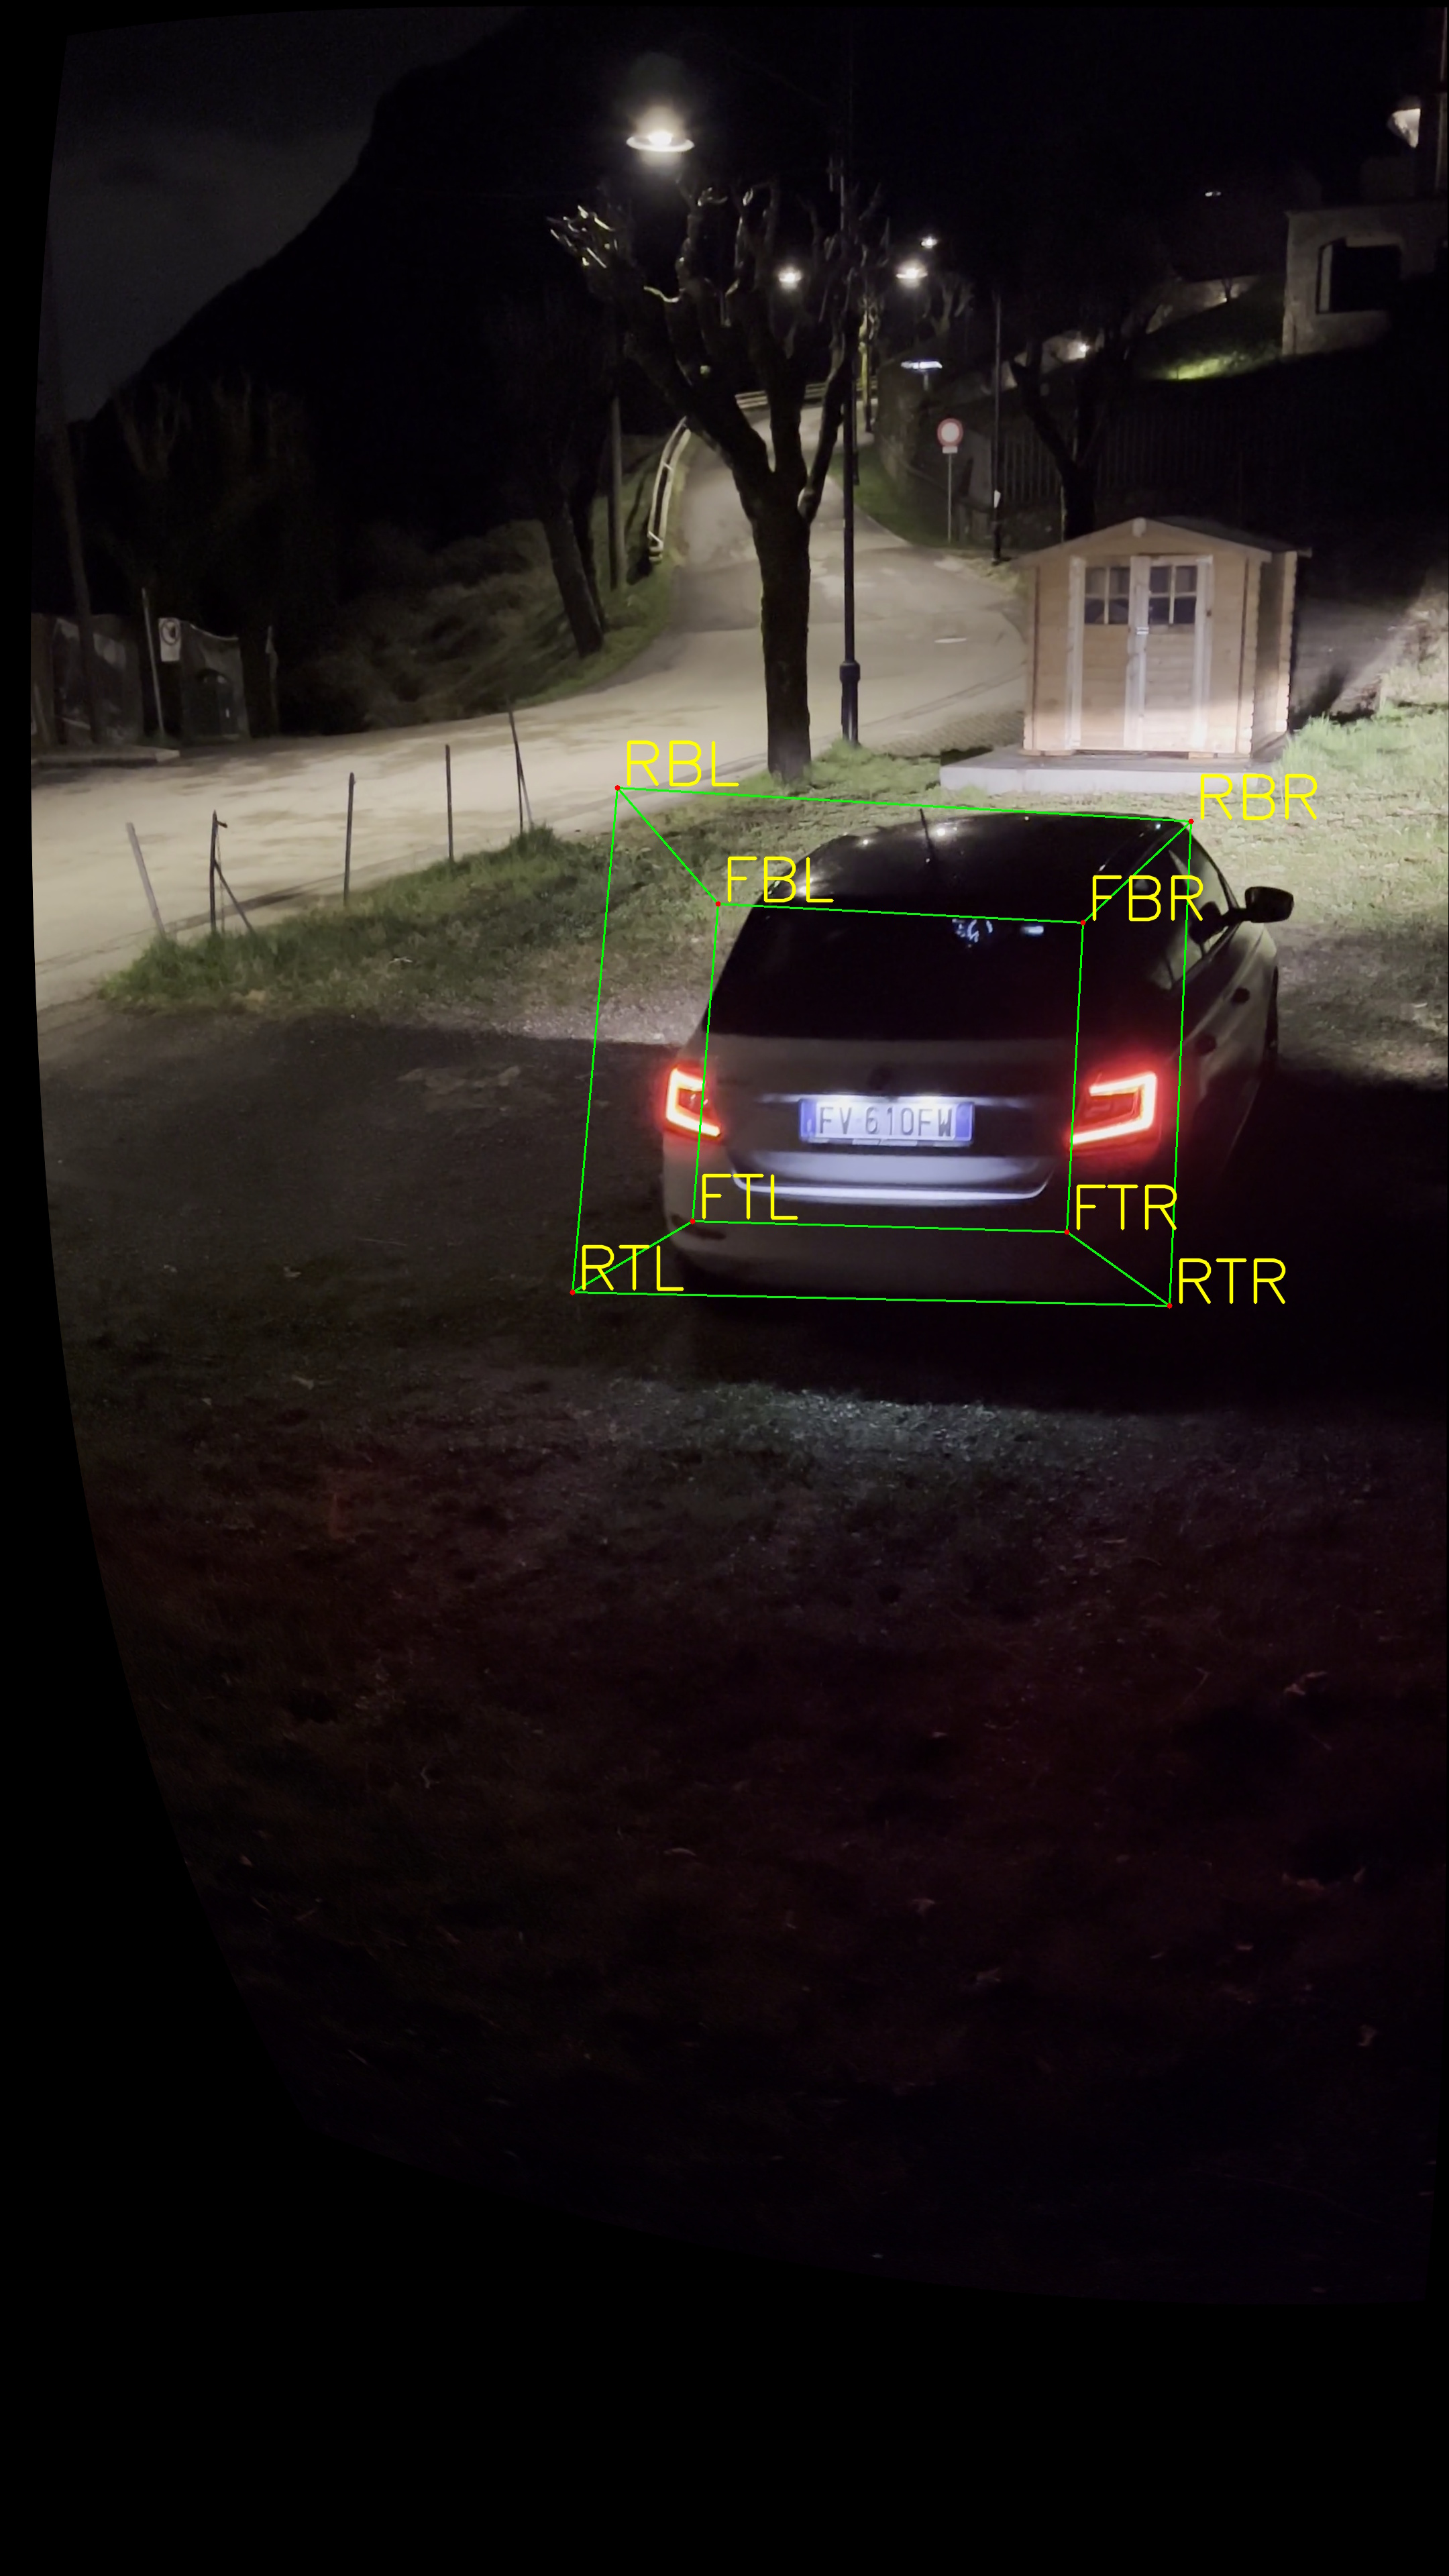
\includegraphics[width=0.30\textwidth]{Images/method1/bbox1.jpg}
    \caption{Projection of the estimated 3D bounding box using the single-frame localization method. Weak perspective and minor feature localization errors affect the accuracy.}
    \label{fig:method1_result}
\end{figure}
